\subsubsection{Composing Structural Patterns}
\label{sec:composing-structural-patterns}

A control flow graph is created by composing various primitive patterns for statements and expressions. The following figures show a couple of examples for common control structures like conditions and loops:

\begin{figure}[h]
  \centering
  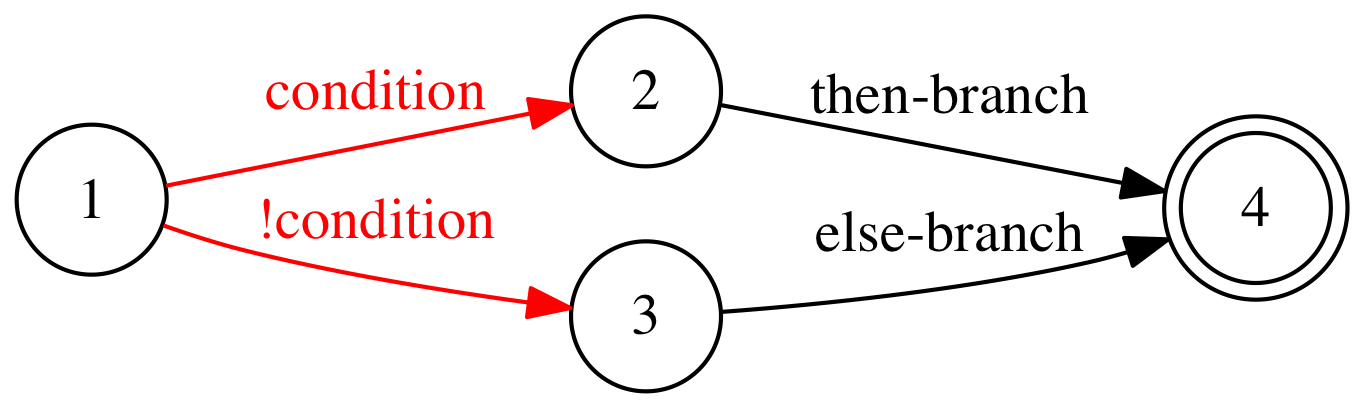
\includegraphics[width=0.7\textwidth]{sections/algorithm/images/if-else}
  \caption{An \code{if}-statement with an \code{else}-block}
  \label{fig:if-else-structural-pattern}
\end{figure}

\begin{figure}[h]
\noindent\begin{minipage}[t]{0.50\textwidth}
  \centering
  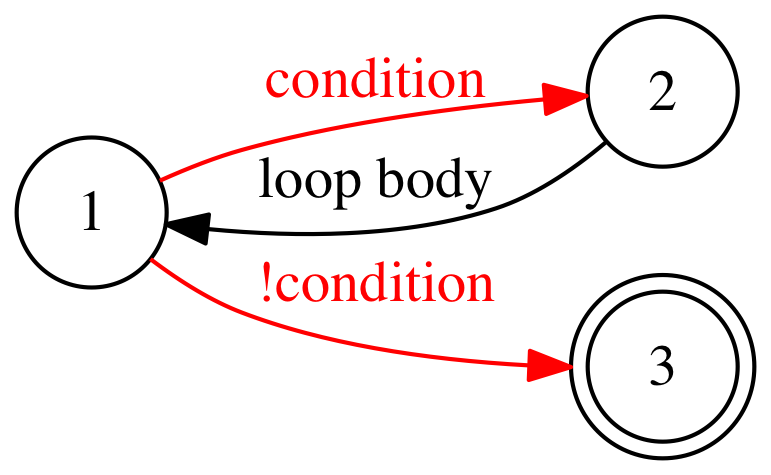
\includegraphics[width=0.8\textwidth]{sections/algorithm/images/while}
  \caption{A \code{while}-loop}
\end{minipage}
\begin{minipage}[t]{0.50\textwidth}
  \centering
  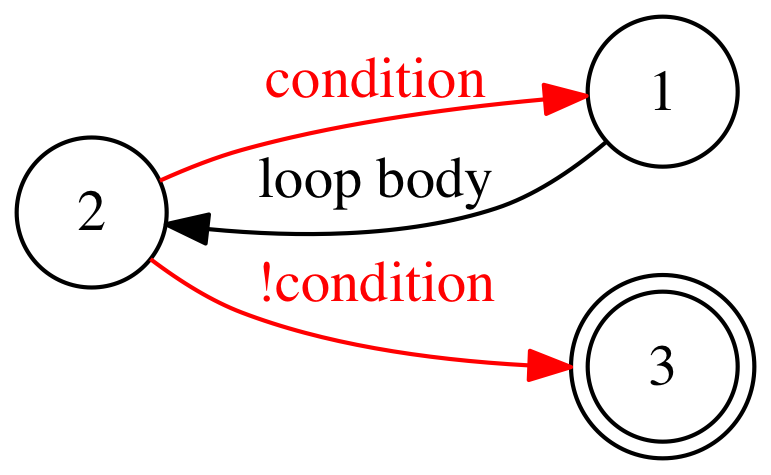
\includegraphics[width=0.8\textwidth]{sections/algorithm/images/do-while}
  \caption{A \code{do-while}-loop}
\end{minipage}
\end{figure}

\begin{figure}[h]
  \centering
  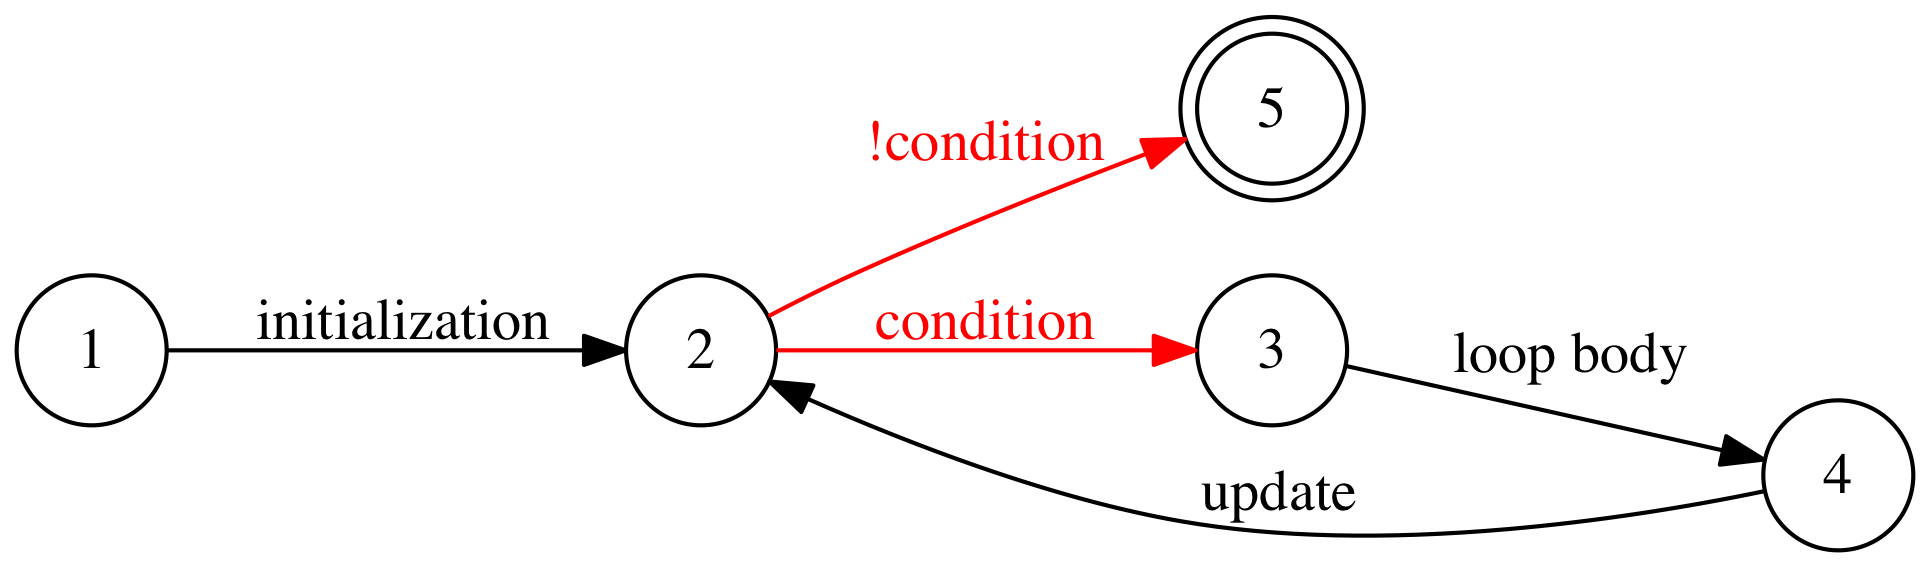
\includegraphics[width=\textwidth]{sections/algorithm/images/for}
  \caption{A \code{for}-loop}
\end{figure}

Each pattern starts with node \#1 and ends with the node that has a double border. In the above figures, those final nodes only have a double border for the purposes of clarification; they are regular nodes in the control flow graph. When two consecutive patterns are combined, the final node of the first becomes the entry node of the second. The black edges that are labeled \emph{then-branch}, \emph{else-branch}, and \emph{loop body} represent the bodies of the control structures. They can consist of arbitrarily many statements, which can contain further nested structures themselves. Similarly, \emph{initialization} and \emph{update} can hold arbitrarily complex expressions. For example, a \code{for}-loop can have a sequence expression like \code{i++, j-{}-} as its update component.

The red edges represent conditional transitions. A node that is not a final node must have either exactly one unconditional outgoing edge or exactly two conditional outgoing edges. For a pair of conditional edges, the condition is evaluated only once. Depending on whether the result is truthy or falsy\footnote{JavaScript has six values that are considered falsy: \code{undefined}, \code{null}, \code{false}, \code{0} (zero), \code{NaN} ("not a number"), and \code{""} (empty string). All other values are considered truthy.}, the corresponding conditional edge is taken.

\nameref{sec:appendix} presents a larger program and its control flow graph.
